\documentclass[12pt]{article}
\usepackage{setspace}
\usepackage{titlesec}
\usepackage{float}
\usepackage{tocloft}
\usepackage{times}
\usepackage[utf8]{inputenc}
\usepackage[margin=1in]{geometry}
\usepackage{apacite}
\usepackage{url}
\usepackage{tikz}
\usepackage{enumitem}
\usepackage{listings}
\usepackage{xcolor}
\usepackage{graphicx}
\usetikzlibrary{arrows.meta, shapes.geometric}

\renewcommand{\baselinestretch}{1.25} 

\titleformat{\section}{\normalfont\Large\bfseries}{\thesection}{1em}{}

\lstset{
  basicstyle=\ttfamily\small,
  keywordstyle=\color{blue},
  stringstyle=\color{red},
  commentstyle=\color{gray},
  numbers=left,
  numberstyle=\tiny,
  stepnumber=1,
  frame=single,
  tabsize=2,
  breaklines=true,
  showstringspaces=false
}

\begin{document}

% Cover Page
\begin{titlepage}
    \centering
    \vspace*{2in}
    {\Huge \bfseries Predicting the Winner of Chess Games Using Binary Classification Machine Learning Models \\[2in]}
    {\Large Seth Schwiethale \\[0.5in]}
    {\Large December 2, 2024 \\}
    \vfill
\end{titlepage}

% Table of Contents
\newpage
\tableofcontents
\newpage

\section{Introduction}
Chess has been one of the world's most popular games for centuries. Over 10 years ago, it was estimated that 605 million adults regularly play chess \cite{fidePressRelease2012}. In the intervening years, the popularity of the game has continued to grow alongside the growth of online gaming where Chess.com alone surpassed 20 million members in 2017 \cite{chessMembers}. With so many chess players around the world, when two meet, how might one predict the winner of the game? This paper compares the application of two Machine Learning binary classification algorithms to this question.

Chess competitions and online platforms commonly use the Elo rating system to indicate the relative skill level of players. Elo ratings can be used to predict the outcome of a match \cite{chessElo}. While Elo ratings are calculated based on the outcomes of previous games, the question is whether a learning algorithm can incorporate additional features of a game to improve upon the prediction accuracy of Elo alone.

To perform this analysis, multiple models were trained using two fundamental supervised classification Machine Learning algorithms: Logistic Regression and Decision Trees. The accuracy of these models were then compared to each other and to the accuracy of predictions made based solely on each player's Elo rating.

\section{Research Background}

\subsection{Elo Ratings and Outcome Prediction}
The Elo rating system was created by Arpad Elo and adopted by the US. Chess Federation in 1960. ``Each player's Elo rating is represented by a number that reflects that person's results in previous rated games. After each rated game, their ratings are adjusted according to the outcome of the encounter.'' \cite{chessElo}. Given the Elo rating of each player, the expected outcome can be calculated with the following formula:


\[
E_A = \frac{1}{1 + 10^{(R_B - R_A)/400}}
\]

Where $E_A$ is the expectation that player $A$ will win and $R_A$ and $R_B$ are the Elo ratings of players $A$ and $B$, respectively. An $E_A$ value $> 0.5$ predicts that will win with increasing probability up to $E_A == 1$.

\subsection{Binary Classification}

In Machine Learning, classification ``is a problem of automatically assigning a label to an unlabeled example'' \cite[Chapter 2, Section 2.7]{100MLB}. If the number of possible labels is two ("White wins", "Black wins"), such a classification problem is called binary classification \cite{Allwein2000}. Though there are three possible outcomes to a chess game: White wins, Black wins or Draw, this study aims specifically to predict a winner, given some set of features describing the characteristics of a specific game, making it a binary classification problem. It is worth noting that, although about 50\% of games end in a draw among the highest-rated players \cite{chessBaseDraws}, most of the world's chess players are not professionals and the occurrence of draws is much lower, less than 5\% in the data used in this analysis.

\subsection{Logistic Regression}

Logistic Regression is a supervised binary classification learning algorithm that uses the standard logistic function, often referred to as the sigmoid function $f_{\textbf{w},b}(\textbf{x})$, whose codomain is $(0, 1)$, to represent the probability that an example is labeled 1. Logistic Regression is trained on a dataset using maximum likelihood optimization by a numerical procedure, such as gradient descent \cite[Chapter 9, Section 9.3]{ShalevShwartz2014}.

\[
f_{\textbf{w},b}(\textbf{x}) := \frac{1}{1 + \exp(-(\langle\textbf{w}, \textbf{x}\rangle + b))}
\]

where $z$ is the inner product of two vectors, the example's features $\textbf{x}$ and the model's learned parameters $\textbf{w}$ plus parameter $b$: $z = \langle\textbf{w}, \textbf{x}\rangle + b$. During training, the log-likelihood $LogL_{\textbf{w},b}$ is maximized for the model's parameters:

\[
LogL_{\textbf{w},b} =
\sum_{i=1}^N y_i\ln{f_{\textbf{w},b}(\textbf{x}) + (1-y_i)\ln(1 - f_{\textbf{w},b}(\textbf{x}))}
\]

\noindent Where $y_i$ is the label for example $i$.

\vspace{12pt}After training, the model has parameters $\textbf{w}$ and $b$ that maximize likelihood that the training dataset is according to the resulting model. These parameters are then used to predict labels for a test set. The results are then used to evaluate the accuracy of the model.

\subsubsection{Considerations}Logistic Regression is sensitive to the scale of features \cite{Alon1997}. Care must be taken when preprocessing the dataset for training to ensure optimal performance.

\subsubsection{Limitations}Logistic Regression is best suited for problems where there is a linear relationship between the features and labels. This may prove to be a limitation when considering the kinds of features available to describe a chess game. Some features, such as opening strategy and game duration may not have a linear relation to the outcomes of the game.

\subsection{Decision Trees}

``A decision tree is an acyclic graph that can be used to make decisions'' \cite[Chapter 3, Section 3.3]{100MLB}. Each branch in a decision tree evaluates a feature in the example and branches left if the value is below a threshold and branches right, otherwise. Decisions trees for classification problems can be constructed by supervised learning. ``The goal is to create a model that predicts the value of a target variable by learning simple decision rules inferred from the data features'' \cite{sklearnDT}. Starting with a root node, the data is split according to each feature and all corresponding thresholds for that feature. The feature and threshold whose resulting split has the largest reduction in entropy (largest information gain) is chosen as the branching feature for that node. The process is repeated recursively to construct the rest of the tree until a stopping condition is met.

Decision tree are easy to visually interpret As shown, in Figure~\ref{fig:decision-tree}, and unlike logistic regression models, decision trees are not sensitive to feature scaling.

\begin{figure}[ht]
\centering
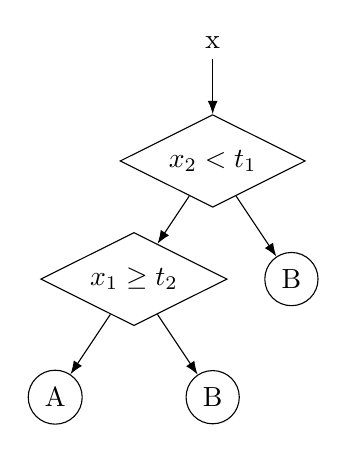
\begin{tikzpicture}[
  edge from parent/.style = {draw, -{Latex}},
  every node/.style = {align=center},
  decision/.style = {draw, diamond, aspect=2, align=center},
  outcome/.style = {draw, circle, align=center},
  level 1/.style = {sibling distance=40mm},
  level 2/.style = {sibling distance=20mm}
]

\node {x}
  child {node[decision] {$x_2 < t_1$} % Left child
    child {node[decision] {$x_1 \ge t_2$} % Left child
      child {node[outcome] {A}}
      child {node[outcome] {B}}
    }
    child {node[outcome] {B}}
  };

\end{tikzpicture}
\caption{A simple decision tree demonstrating decision and leaf nodes.}
\label{fig:decision-tree}
\end{figure}

\subsubsection{Considerations}Decision trees can be biased (over-fitting) if trained on unbalanced examples. Care must be taken to balance the dateset in preprocessing to reduce bias in the decision tree model.

\subsubsection{Limitations}Decision trees can become complex and are prone to over-fitting the training data.

\subsection{Related Work}
Historically, sports and game prediction models used statistical approaches - e.g. \cite{Clarke1995} \cite{Bailey2006}. But around the 2010s, as datasets grew even with comparatively-scarce computational resources \cite{Bottou2003}, the popularity of machine learning for the domain of sports analysis experienced a significant rise \cite{aiSports} with the publishing of seminal papers \cite{Constantinou2012} that influenced sports betting strategies.

The use of logistic regression for prediction models has been explored by many researchers, because ``A common type of prediction problem is generalized linear regression, which includes linear regression, logistic regression, other generalized linear models'' \cite{Gordon1999}. Particularly of relevance to this research, logistic regression has been used to predict outcomes in many games, such as European-Football \cite{Prasetio2016}, where the authors achieved 69\% accuracy with just a few features and Ice Hockey \cite{Chin2023}, where logistic regression models outperformed Decision Tree, Support Vector Machine and Artificial Neural Network models used as benchmarks from prior work \cite{Pischedda2014} \cite{Igiri2014}.

Decision Trees have also been researched in relation to predicting the outcome of other games, such as Cricket \cite{Kumar2018}, where the authors' decision tree model had an accuracy of $55.1\%$ and football \cite{Jaeyalakshmi2023}, where the authors built a model with $67.9\%$ accuracy.

A search for prior research of machine learning techniques applied to chess generally yielded research focused on creating chess-playing engines, AI that can predict the best next move for in-game competitve play; a problem not closely related to the aim of this research. This paper evaluates logistic regression and decision trees in a way that is similar to the research referenced above, but applied to the game of chess, which differs in many ways from the sports for which most similar analysis has been done.

\section{Materials and Data Sources}
\label{sec:dataset}

Training and assessment of the chosen model types was performed using the Chess Game Dataset published at kaggle.com \cite{chessDataset}. The dataset contains just over 20,000 games that were collected from the open-source online chess game server Lichess.org \cite{lichessOrg}. The dataset contains 16 raw features or columns with no missing values, Table~\ref{tab:features}.

\subsection{Available Features}
\label{sec:features}

\begin{table}[H]
\centering
\begin{tabular}{|l|l|}
\hline
$\textbf{Feature}$ & Description \\ \hline
$\textbf{Game ID}$ & A unique string to identify a game \\ \hline
$\textbf{Rated (T/F)}$ & True if the game was rated \\ \hline
$\textbf{Start Time}$ & A time stamp indicating when the game began \\ \hline
$\textbf{End Time}$ & A time stamp indicating when the game ended \\ \hline
$\textbf{Number of Turns}$ & How many turns were made before the game ended \\ \hline
$\textbf{Victory Status}$ & A string describing how the game ended \\ \hline
$\textbf{Winner}$ & A string representing the winner of the game by color, if any \\ \hline
$\textbf{Time Increment}$ & A string representing how the game was timed \\ \hline
$\textbf{White Player ID}$ & A string unique to a player \\ \hline
$\textbf{White Player Rating}$ & Elo rating for player \\ \hline
$\textbf{Black Player ID}$ & A string unique to a player \\ \hline
$\textbf{Black Player Rating}$ & Elo rating for player \\ \hline
$\textbf{Moves}$ & All Moves in Standard Chess Notation \\ \hline
$\textbf{Opening Eco}$ & Standardized Code for any given opening strategy \\ \hline
$\textbf{Opening Name}$ & A string representing the opening strategy \\ \hline
$\textbf{Opening Ply}$ & Number of moves in the opening phase \\ \hline
\end{tabular}
\caption{Available features in dataset.}
\label{tab:features}
\end{table}

\subsection{General Preprocessing}
As detailed below, different data preprocessing steps were performed for each learning algorithm, but in both cases, games with no winner were filtered from the dataset, leaving 19,108 examples. Additionally, the following features were either not included in either training dataset or were transformed:

\begin{itemize}[label={}, leftmargin=0pt]
  \item $\textbf{Drop: id}$ - The Game ID column is a unique identifier and doesn’t provide any predictive value. Including this feature would surely contribute to over-fitting, since this unique set of values only exists in the training set.
  \item $\textbf{Drop: increment\_code}$ - This feature was mistakenly interpreted as the change in Elo rating after the game, so it was not included. Further discussion can be found in Section~\ref{sec:discussion}.
  \item $\textbf{Drop: white\_id and black\_id}$ - The specific goal of the research was to evaluate models that can generalize well, without knowing specifically who the player is.
  \item $\textbf{Transform: created\_at and last\_move\_at}$ - The start and end time were decided to be less predictive than the duration of a game, so these two columns were transformed into a new column: $\textbf{duration}$.
  \item $\textbf{Drop: moves}$ - The moves column contains move sequences, which are high-dimensional and computationally expensive to process for simple predictions. Further discussion can be found in Section~\ref{sec:discussion}.
  \item $\textbf{Drop: opening\_name}$ - Redundant interpretation of $\textbf{opening\_eco}$.
  \item $\textbf{Transform: white\_player\_rating and black\_player\_rating}$ - Convert these features to a single feature which is the difference between the two players' ratings: $\textbf{rating\_diff}$. Positive numbers mean white has a higher rating and negative numbers mean black has a higher rating.
\end{itemize}

\section{Research and Methods}
\label{sec:methods}
For this research, implementations of logistic regression and decision tree learning algorithms from scikit learn, the Python machine learning library, were used. Before training each model, some preprocessing of data was performed to optimize the performance of the respective learning algorithm. For each algorithm, multiple models were trained with varying feature sets. For decision trees, the hyper-parameters were also tuned for optimal performance. Each model was evaluated by the metrics: Accuracy, precision, recall and F1 Score. The most accurate model from each algorithm is compared in Section~\ref{sec:results}.

\subsection{Logistic Regression Model Training}

\subsubsection{Data Preprocessing}

\noindent\textbf{Encoding and Normalizing Numerical Features}

In order to optimize the performance of the logistic regression learner, the following steps were taken to preprocess the dataset before training. Generally, this included: removing columns with no meaningful predictive value for this research's purpose, encoding string-based features to numerical features on a case-by-case basis, normalizing resulting features and checking for multicollinearity among remaining features.


\begin{itemize}[label={}, leftmargin=0pt]
  \item $\textbf{Normalize: rating\_diff, turns, duration}$ - Normalize features by scaling between 0 and 1, using Z-Score, to improve model performance.

  \begin{lstlisting}[language=Python, caption={example: normalizing ratings}]
    # create a new column for rating difference
    df['rating_diff'] = df['white_rating'] - df['black_rating']
    # normalize with Z-Score
    # calculate mean and standard deviation for rating_ddiff
    rating_diff_mean = df['rating_diff'].mean()
    rating_diff_std = df['rating_diff'].std()
    # normalize rating_diff
    df['rating_diff_normalized'] = (df['rating_diff'] - rating_diff_mean) / rating_diff_std
  \end{lstlisting}

  \item $\textbf{Encode: opening\_eco}$ - The opening ECO feature represents chess opening strategies coded with a classification system. To utilize this feature in a logistic regression learner, it was decided to convert each code instance to a count of how many times that opening was used in the dataset. This new feature can be thought of as the opening's popularity. The newly encoded opening ECO was finally normalized. Other encodings for this feature can be imagined, such as ranking openings by how often they resulted in a win for white.
\end{itemize}

\noindent\textbf{Reducing Multicollinearity}

Next, the preprocessed features were analyzed for multicollinearity with a correlation matrix, as shown in Figure~\ref{fig:corr-matrix-1}.

\begin{figure}[H]
\centering
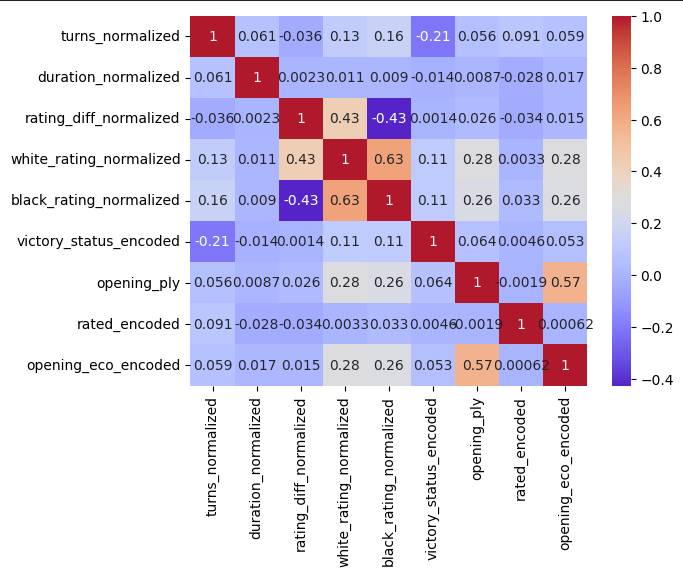
\includegraphics[width=0.8\textwidth]{corr-matrix-1.png}
\caption{Initial Correlation Matrix for Logistic Regression Features}
\label{fig:corr-matrix-1}
\end{figure}

The ratings for black and white players were unsurprisingly correlated (in online games, players of similar experience tend to play each other). These features were not used to train the model. The rating difference between players was used, instead.

$\textbf{opening\_eco\_encoded}$ and $\textbf{opening\_ply}$ are also moderately correlated, so PCA was applied to reduce dimensionality in the data set. The principal component of these two features was given the name $\textbf{pca\_opening\_features}$. The resulting correlation matrix is shown in Figure~\ref{fig:corr-matrix-2}.

\begin{figure}[H]
\centering
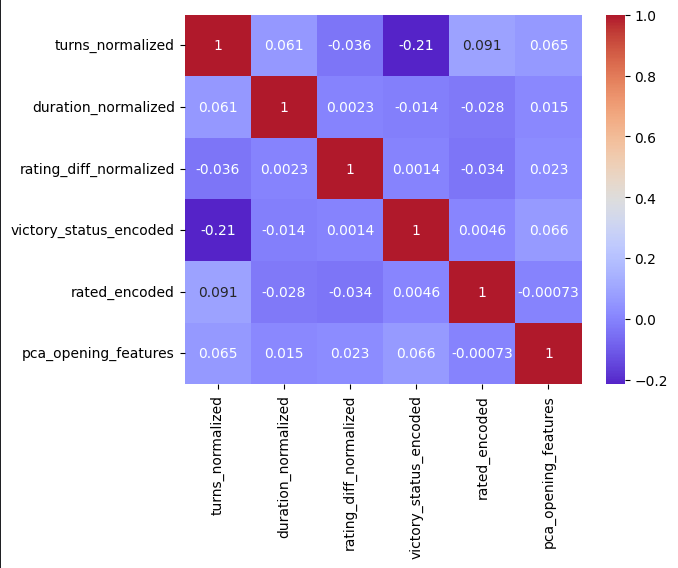
\includegraphics[width=0.8\textwidth]{corr-matrix-2.png}
\caption{Final Correlation Matrix for Logistic Regression Features}
\label{fig:corr-matrix-2}
\end{figure}

\subsubsection{Training and Evaluation}

The dataset was split into training and testing sets, 80\% and 20\%, respectively. The scikit-learn LogisticRegression implementation was used to fit the models to the training data. Many models were produced, each using a different set of features. Each model was evaluated with the testing set, using the metrics: Accuracy, precision, recall and F1 Score.

\subsection{Decision Tree Model Training}

\subsubsection{Data Preprocessing}
Less preprocessing was required for the decision tree learner than was for the logistic regression learner because decision trees are not sensitive to feature scaling. However, while decision trees can theoretically handle both numerical and categorical data, the scikit-learn implementation does not support categorical variables \cite{sklearnDT} (scikit-learn uses an optimized version of CART \cite{classificationTrees1984}), so features of interest with categorical representations were encoded with an appropriate numerical representation.

\begin{itemize}[label={}, leftmargin=0pt]
  \item \textbf{Encode: rated} - boolean feature encoded to $False \rightarrow 0$ and $True \rightarrow 1$
  \item \textbf{Encode: winner} - label encoded to $white \rightarrow 0$ and $black \rightarrow 1$
  \item $\textbf{Encode: opening\_eco}$ - The opening ECO feature represents chess opening strategies coded with a classification system. To utilize this feature in a decision tree learner, as in the logistic regression case, it was decided to convert each code instance to a count of how many times that opening was used in the dataset. This new feature can be thought of as the opening's popularity. 
\end{itemize}

\subsubsection{Training and Evaluation}
The dataset was split into training and testing sets, 80\% and 20\%, respectively. The scikit-learn DecisionTree implementation was used to fit the models to the training data. Many models were produced, each using a different set of features. Additionally, the scikit-learn's $GridSearchCV$ \cite{sklearnGSCV} algorithm was used to perform an exhaustive search for optimum hyper-parameters: $max\_depth$, $min\_samples\_split$, $min\_samples\_leaf$ and $max\_features$. Each model was evaluated with the testing set, using the metrics: Accuracy, precision, recall and F1 Score.


\section{Results}
\label{sec:results}

\subsection{Predicting with Elo Rating as Baseline}
To evaluate each model's predictive power, predictions based solely on players' Elo rating were used as a baseline. 

\subsubsection{Method}
This baseline evaluation was performed over the entire dataset, minus rows with no winner. The heuristic used was simply:

\begin{itemize}
  \item If \textit{rating\_diff} is positive or zero $\rightarrow$ predict \textbf{White Wins}
  \item If \textit{rating\_diff} is negative $\rightarrow$ predict \textbf{Black Wins}
\end{itemize}

 Recall how the \textit{rating\_diff} feature was encoded: $\textit{white\_rating} - \textit{black\_rating}$. This heuristic simply predicts that the player with the highest Elo rating will win. If players have equal ratings, there is assumed to be a first-move advantage \cite{Streeter1946}, giving white the edge.

\subsubsection{Evaluation}

\begin{table}[h!]
\centering
\begin{tabular}{|l|l|}
\hline
$\textbf{Accuracy}$ & $0.651$ \\ \hline
$\textbf{Precision}$ & $0.65$ \\ \hline
$\textbf{Recall}$ & $0.65$ \\ \hline
$\textbf{F1 Score}$ & $0.65$ \\ \hline
\end{tabular}
\caption{Elo Heuristic Baseline.}
\label{tab:el-baseline}
\end{table}

\begin{figure}[H]
\centering
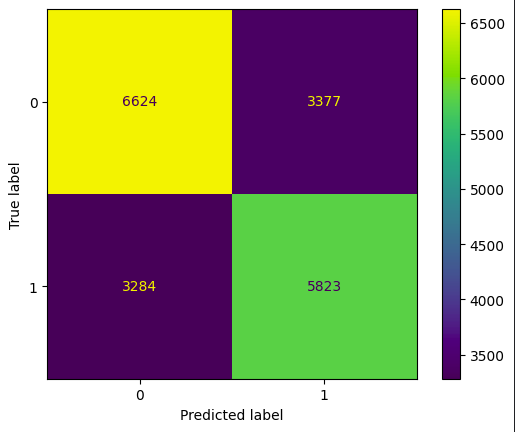
\includegraphics[width=0.8\textwidth]{conf-matrix-elo.png}
\caption{Confusion Matrix for Elo Heuristic.}
\label{fig:conf-matrix-elo}
\end{figure}

\subsection{Logistic Regression}

\subsubsection{Method}
Several Models with differing sets of features were trained and evaluated. The model with the highest accuracy was trained with the following features:

\begin{itemize}
  \item\textit{turns\_normalized}
  \item\textit{duration\_normalized}
  \item\textit{rating\_diff\_normalized}
  \item\textit{rated\_encoded}
  \item\textit{pca\_opening\_features}
\end{itemize}

\subsubsection{Evaluation}

\begin{table}[h!]
\centering
\begin{tabular}{|l|l|}
\hline
$\textbf{Accuracy}$ & $0.655$ \\ \hline
$\textbf{Precision}$ & $0.66$ \\ \hline
$\textbf{Recall}$ & $0.66$ \\ \hline
$\textbf{F1 Score}$ & $0.66$ \\ \hline
\end{tabular}
\caption{Logistic Regression Model Evaluation.}
\label{tab:lr-eval}
\end{table}

\begin{figure}[H]
\centering
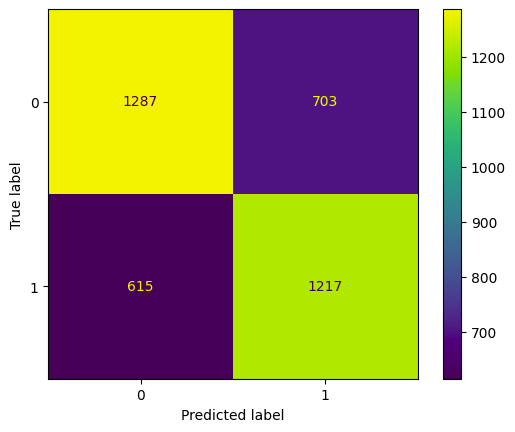
\includegraphics[width=0.8\textwidth]{conf-matrix-logit.png}
\caption{Confusion Matrix for Logistic Regression Model.}
\label{fig:conf-matrix-logit}
\end{figure}

\subsection{Decision Trees}

\subsubsection{Method}
Many Decision Tree models were built, trained with different sets of features and hyperparameter values. The model with the highest accuracy was trained with the following features and hypervalues:

\begin{itemize}
  \item\textbf{Feature}: \textit{turns}
  \item\textbf{Feature}: \textit{rated\_encoded}
  \item\textit{max\_depth}: \textbf{None}
  \item\textit{max\_features}: \textbf{None}
  \item\textit{min\_samples\_leaf}: \textbf{$5$}
  \item\textit{min\_samples\_split}: \textbf{$2$}
\end{itemize}

\subsubsection{Evaluation}

\begin{table}[h!]
\centering
\begin{tabular}{|l|l|}
\hline
$\textbf{Accuracy}$ & $0.796$ \\ \hline
$\textbf{Precision}$ & $0.80$ \\ \hline
$\textbf{Recall}$ & $0.80$ \\ \hline
$\textbf{F1 Score}$ & $0.80$ \\ \hline
\end{tabular}
\caption{Decision Tree Model Evaluation.}
\label{tab:dt-eval}
\end{table}

\begin{figure}[H]
\centering
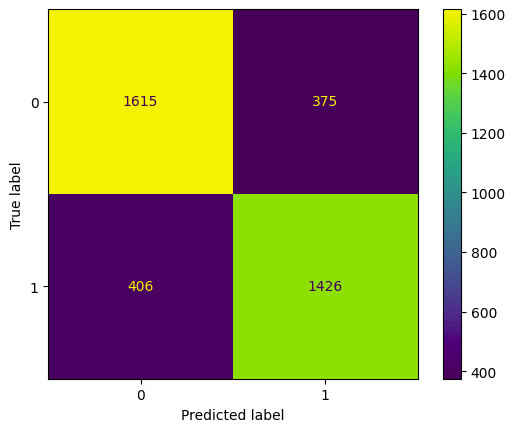
\includegraphics[width=0.8\textwidth]{conf-matrix-dt.png}
\caption{Confusion Matrix for Decision Tree Model.}
\label{fig:conf-matrix-dt}
\end{figure}


\section{Discussion and Conclusions}
\label{sec:discussion}

The aim of this research was to evaluate whether a machine learning algorithm could incorporate features of a chess game to improve upon the outcome prediction accuracy of Elo ratings alone. First, the accuracy of an Elo rating-based heuristic was assessed using the Chess Game Dataset (Lichess), detailed in Section~\ref{sec:dataset}. Next, to accomplish the goal of this effort, two classification learning algorithms were explored: logistic regression and decision trees. As detailed in Section~\ref{sec:methods}, many models were built, using varying feature sets and hyper-parameter values, to yield candidate models with the best accuracy. No logistic regression model was found to improve upon the Elo heuristic approach. However, decision tree models were trained with higher outcome prediction accuracy, the best of which yielding an F1 Score of $80\%$ when evaluated with the testing portion of the dataset.

These results suggest that supervised machine learning algorithms can in fact be trained to make more accurate chess game outcome predictions than predicting the outcome based solely on Elo ratings. The implications of these results present both limitations and opportunities, which are discussed below.

\subsection{Limitations to approach}

\subsubsection{Features Used Entail the Game has Ended}
Most of the features available for training had a temporal dimension, meaning they represented information known only after a game had begun (e.g. \textbf{Opening ECO}) or ended (e.g. \textbf{Number of Turns}). While this research demonstrated that incorporating details about a game in addition to the players' Elo ratings could yield more accurate outcome predictions, the models that were produced generally rely on the fact that the game has been concluded. This assumption places constraints and limitations on the practical application of such models. One can imagine outcome prediction applications that are relevant only before a game has occurred or ended, such as estimating betting odds. The models produced in this research would not have value for such applications. However, this observation does not preclude the possibility of identifying other game features that may be successfully used to train models designed for these applications, but further research would be required. Specific considerations are detailed in Section~\ref{sec:feature-eng}.

\subsubsection{Correlation of Draw Occurrence and Player Rating}
As previously noted, as the ratings of players increase to master level, the occurrence of draw outcomes greatly increases. This research limited its models to binary classifiers, focusing solely on models that would produce a winner. Such models are inherently less-accurate when the Elo ratings of players are exceptionally high. Multi-class classifier models would likely be needed to account for this phenomenon. Specific considerations are detailed in Section~\ref{sec:multiclass}.

\subsection{Future Work}

\subsubsection{Additional Feature Selection and Engineering}
\label{sec:feature-eng}
Some of the features available in this dataset could provide additional predictive utility before a game has concluded. In particular, the \textbf{Moves} feature (Section~\ref{sec:features}) was not utilized in this research. One could imagine that as the game develops, advantages may become more apparent. Perhaps a model limited to incorporating the first 10 moves could have improved predictive accuracy without relying on features only present at the conclusion of the game.

Another example of a feature in this dataset that could be explored further is \textbf{Opening ECO} (Section~\ref{sec:features}). For this research, the feature was encoded from a coded label of the specific strategy to the strategy's popularity in the dataset. During the analysis of these research results, it was considered that a better approach may have been to encode this field according to the relative success of the strategy. For example, strategies could have been encoded with a numerical rank that corresponded to how often the strategy resulted in a win for white. Additional encodings could be considered and evaluated.

Finally, other datasets exist (e.g. Chess Base Database with over 8 million games \cite{chessBaseDb}) and may contain features that provide a better training environment. More rigorous approaches could be taken to select the most important features from an abundant set of irrelevant features (as a classic example, Winnow \cite{Littlestone1988}).

\subsubsection{Multi-class Models}
\label{sec:multiclass}
To improve accuracy, especially when predicting the outcome of chess games between higher-rated players, multi-class classifiers could be trained to include the three possible chess game outcomes: \textbf{White Wins}, \textbf{Black Wins} and \textbf{Draw}. To accomplish this, a larger dataset would be required; one that includes more games from players of higher rating to provide balanced examples of all outcomes (the dataset used for this research contained less than $5\%$ draws). Such an expanded dataset may present its own challenges, such as introducing bias toward more-advanced game play (models trained mostly on master-level games would not generalize well for lower-level players).

\subsubsection{Explore Additional Machine Learning Algorithms}
This research was limited to the exploration of two fundamental supervised machine learning classification models. Further research could investigate more advanced models, including but not limited to deep neural networks and ensemble learners.

\subsubsection{Deep Neural Networks}
With access to more compute power and one of the larger datasets available, datasets with millions of examples, it may be beneficial to try using a deep neural network. Deep Neural Networks may also provide benefits when considering high-dimensional dataset, such as the approach proposed in Section~\ref{sec:multiclass}.

\subsubsection{Ensemble Learning}
Ensemble Learners could be used to improve the accuracy of the algorithms explored in this research while reducing variance and bias \cite[Chapter 7, Section 7.5]{100MLB}. "Boosting" algorithms combine several weak learners, which approximate the unknown target function and boost or amplify the weak learners to achieve higher levels of accuracy \cite{Kearns1996}. Gradient Boosting is a popular example of such an algorithm and can handle large, high-dimensional datasets and produce very accurate models \cite{greeksGeeksGB}. This algorithm has promise to further improve on the decision tree approach used in this research

% References in APA format
\newpage
\bibliographystyle{apacite}
\bibliography{references}  % Ensure there is a file named references.bib with your bibliography entries.

\end{document}